\documentclass[12pt]{article}
%---DOCUMENT MARGINS---
\usepackage{geometry} % Required for adjusting page dimensions and margins
\geometry{
	paper=a4paper, % Paper size, change to letterpaper for US letter size
	top=4cm, % Top margin
	bottom=2cm, % Bottom margin
	left=2cm, % Left margin
	right=2cm, % Right margin
	headheight=3cm, % Header height
	%footskip=1.5cm, % Space from the bottom margin to the baseline of the footer
	headsep=0.5cm, % Space from the top margin to the baseline of the header
	%showframe, % Uncomment to show how the type block is set on the page
}
\usepackage{cmap}

\usepackage[T2A]{fontenc}
\usepackage[bulgarian]{babel}
\usepackage{fontspec}
\setmainfont{Times New Roman}
\setsansfont{Times New Roman}
\setmonofont{Courier New}
\usepackage[math-style=TeX]{unicode-math}
\setmathfont{Latin Modern Math}

\usepackage[nobottomtitles*]{titlesec}
\titleformat
{\section} % command
{\normalfont\fontsize{14}{14}\sffamily\bfseries} % format
{} % label
{0pt} % sep
{} % before-code
\titlespacing{\section}{0pt}{0em}{0em}
\newcommand{\problem}[1]{%
	\section[#1]{#1 \fontsize{12}{12}{\hfill{\normalfont{
				\emoji{hourglass-not-done}\tl \space\space \emoji{floppy-disk} \ml}}}}
}
\usepackage[dvipsnames]{xcolor}
\titleformat
{\subsection} % command
{\fontsize{14}{14}\itshape} % format
{} % label
{0pt} % sep
{} % before-code
[\vspace{-1em}{\color{LimeGreen}\rule{0.2\textwidth}{0.2em}}\vspace{-0.7em}] % after-code
\titlespacing{\subsection}{0pt}{0.5em}{0em}

\setlength{\parskip}{0.5em}
\setlength{\parindent}{24pt}
\sloppy

\usepackage{fancyhdr}
\pagestyle{fancy}
\usepackage{setspace}
\fancyhead[L]{
	\begin{minipage}{\textwidth}
		
\includegraphics[width=2.5cm]{./logo.jpg}
	\end{minipage}
}
\fancyhead[C]{
	\begin{minipage}{\textwidth}
		\centering\large\bf{\header}
		\vspace{-0.35cm}
	\end{minipage}
}
\fancyhead[R]{}
\renewcommand{\headrulewidth}{0cm}
\fancyheadoffset[L,R]{1cm}
\usepackage{lastpage}
\fancyfoot[C]{\thepage\ / \pageref*{LastPage}}

\raggedbottom

\usepackage{amsmath}
\usepackage{stmaryrd}

\usepackage{graphicx}
\graphicspath{{./}}
\usepackage[export]{adjustbox}
\usepackage{wrapfig}
\makeatletter
\patchcmd\WF@putfigmaybe{\lower\intextsep}{}{}{\fail}
\AddToHook{env/wrapfigure/begin}{\setlength{\intextsep}{0pt}}
\makeatother
\usepackage[inkscapearea=page,inkscapepath=./svg-inkscape]{svg}
\svgpath{{./}}

\usepackage{makecell}
\usepackage{tabularray}
\AtBeginEnvironment{table}{\vspace{-0.2cm}}
\AtEndEnvironment{table}{\vspace{-0.2cm}}
\usepackage{float}
\usepackage{placeins}
\usepackage{caption}
\captionsetup[table]{
	skip=0.25em,font=it,
	singlelinecheck=false,justification=justified,indention=-24pt,
	margin={24pt, 0pt}
}

\usepackage{enumitem}
\setlist{itemsep=-0.4em,leftmargin=\parindent,topsep=-\parskip}
\newcommand{\tabitem}{\indent~~\llap{\textbullet}~~}

\usepackage{hyperref}
\hypersetup{
	colorlinks=true,
	citecolor=blue,
	linkcolor=blue,
	urlcolor=cyan,
}

\usepackage{emoji}
\renewcommand{\bottomtitlespace}{3cm}

\newcommand{\header}{
	ПРОЛЕТНИ СЪСТЕЗАНИЯ ПО ИНФОРМАТИКА\\
	Шумен, 19 – 21 април 2024 г.\\
	Група B, 9 – 10 клас
}
\begin{document}

\newcommand{\tl}{$0.8$ сек.}
\newcommand{\ml}{$256$ MB}
\problem{Задача B2. ИЗБЯГАЙ}

Сашка, Давко Дамянов и Вие се намирате в отборна словенска напредавара по Ескейп стаи. Ескейп стаята, в която се намирате, може да се опише като мрежа от $N$ помещения, номерирани с числата от $1$ до $N$, свързани с двупосочни $M$ коридора между тях, номерирани с числата от $1$ до $M$. Всеки коридор има трудност за преминаване от $1$ до $26$, като трудностите са означени с малки букви от латинската азбука, където $a$ е най-малката, а $z$ -- най-голямата трудност. Така $i$-тият коридор свързва $u_i$-тото и $v_i$-тото помещение, като има трудност за преминаване $l_i$. Няма коридор, който да свързва помещение със себе си, и няма два различни коридора, свързващи една и съща двойка помещения. Макар и да имат различни трудности, коридорите се изминават за едно и също време. Сашка започва в помещение $№1$ и се цели да достигне изхода, намиращ се в помещение $№N$.

Сашка има много опит в Ескейп стаите, до толкова, че тя винаги минава по маршрута с най-малко времетраене. Освен това, тя иска да запази интересното за най-накрая, заради това се стреми да измине \textit{лексикографски най-малкия} маршрут, измежду тези с най-малко времетраене.

Сашка обаче би се чувствала гузно, ако свърши всичко сама. Заради това тя се обръща към Вас да напишете програма \textbf{\texttt{escape}}, която да намери една такава последователност от коридори $p_1,p_2,...,p_k$, по която момичето да премине.

\subsection{Формална дефиниция}
Поредица от коридори с номера $p_1,p_2,...,p_k$ е валиден маршрут, когато:

\begin{itemize}
    \setlength{\itemindent}{12pt}
    \item $1 \in \{u_{p_1}, v_{p_1}\}$
    \item $N \in \{u_{p_k}, v_{p_k}\}$
    \item $\{u_{p_i}, v_{p_i}\} \cap \{u_{p_{i+1}}, v_{p_{i+1}}\} \neq 	\varnothing\ $ за $ \forall i \in [1, k - 1]$.
    \item $\{u_{p_i}, v_{p_i}\} \cap \{u_{p_{i+1}}, v_{p_{i+1}}\} \neq 	\{u_{p_{i+1}}, v_{p_{i+1}}\} \cap \{u_{p_{i+2}}, v_{p_{i+2}}\}$ за $ \forall i \in [1, k - 2]$.
    \item $k$ е минималното възможно от всички коридори, спазващи горните условия.
    \item Нека цената на маршрута $f(p_1,p_2,p_3,...,p_k)=l_{p_1} + l_{p_2} + l_{p_3} + ... + l_{p_k}$, където $+$ е знак за конкатенация. $f(p_1,p_2,p_3,...,p_k)$ е лексикографски най-малкият низ от множеството на всички низове, образувани от маршрути, изпълняващи горните условия.
\end{itemize}

\vspace{12pt}

Един низ $a_1,a_2,...,a_k$ е лексикографски по-малък от друг низ $b_1,b_2,...,b_k$, ако съществува позиция $x$, $(x \leq k)$, за която:
\begin{itemize}
    \setlength{\itemindent}{6pt}
    \item $a_i = b_i$ за $1 \leq i < x$.
    \item $a_x$ е по-напред в латинската азбука от $b_x$.
\end{itemize}

\vspace{6pt}

Един низ $a$ е лексикографски най-малък от дадено множество от низове, ако в това множество няма низ, който да е лексикографски по-малък от $a$.

\vspace{12pt}

\subsection{Вход}
На първия ред от стандартния вход са дадени две цели числа, съответно $N$ и $M$. На останалите $M$ реда от стандартния вход са характеризирани $M$-те коридора, като на $i$-тия ред са дадени $u_i$, $v_i$ и $l_i$.

\subsection{Изход}
На стандартния изход отпечатайте получения низ $f(p_1,p_2,...,p_k)$ т.е. трудностите на коридорите в реда на преминаването по тях, зададен според най-добрия маршрут (или един от най-добрите такива).
 
\subsection{Ограничения}
\vspace{0.1em}
\begin{itemize}
	\item $2 \leq N \leq 300\ 000$
	\item $1 \leq M \leq 600\ 000$
    \item $1 \leq u_i, v_i \leq N$
    \item $l_i \in \{a, b, ..., z\}$
    \item $u_i \neq v_i\ (1 \leq i \leq M)$
    \item $(u_i,v_i) \neq (u_j,v_j)$ и $(u_i,v_i) \neq (v_j,u_j)\ (1 \leq i < j \leq M)$
    \item Може да се стигне от всяка стая до всяка друга посредством коридорите. 
\end{itemize}

\subsection{Подзадачи}
\begin{table}[ht]
	\begin{tblr}{|X[14,c,m]|X[16,c,m]|X[11,c,m]|X[11,c,m]|X[11,c,m]|X[23,c,m]|}
		\hline
		\textbf{Подзадача} & \textbf{Необходими подзадачи} & \textbf{Точки} & $N$ & $M$ & \textbf{Други ограничения}\\
		\hline
		  $1$ & -- & $0$ & -- & -- & Примерния тест. \\ 
		\hline
		  $2$ & -- & $11$ & $\leq 300\ 000$ & $\leq 600\ 000$ & $l_i=a$ \\ 
		\hline
		  $3$ & $1$ & $22$ & $\leq 1\ 000$ & $\leq 2\ 000$ & -- \\ 
		\hline
            $4$ & $1;3$ & $37$ & $\leq 100\ 000$ & $\leq 200\ 000$ & -- \\
		\hline
            $5$ & $1-4$ & $30$ & $\leq 300\ 000$ & $\leq 600\ 000$ & -- \\
		\hline
	\end{tblr}
	\caption*{Точките за дадена подзадача се получават само ако се преминат успешно всички тестове, предвидени за нея.}
\end{table}
\FloatBarrier
\vspace{-6pt}
\subsection{Пример}
\begin{table}[ht]
	\begin{tblr}{|X[17,l]|X[17,l]|X[66,j]|}
		\hline
		\textbf{Вход} & \textbf{Изход} & \textbf{Обяснение на примера} \\
		\hline
		\texttt{8 10\\
                    1 2 a\\
                    1 3 a\\
                    2 4 c\\
                    3 4 b\\
                    3 5 b\\
                    4 6 a\\
                    4 7 a\\ 
                    5 6 b\\
                    7 8 b\\ 
                    6 8 b} & 
            \texttt{abab}
		& 
		{Ескейп стаята е показана на изображението.\\
		\begin{adjustbox}{width=0.55\textwidth, valign=t, center, margin=0cm 0.1cm 0cm 0.1cm}
			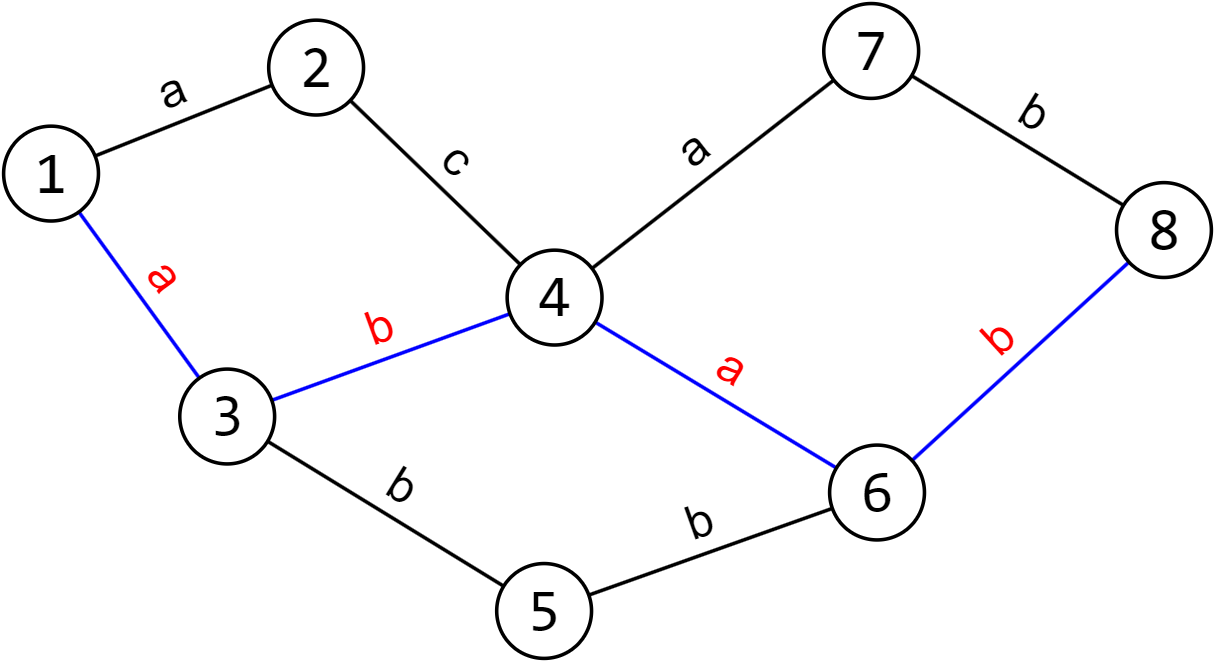
\includegraphics{exampleEscape.png}
		\end{adjustbox}} \\ \\
		\hline
	\end{tblr}
\end{table}

\end{document}
